\documentclass[12pt,a4paper]{article}
\usepackage[utf8]{inputenc}
\usepackage[T1]{fontenc}
\usepackage{amsmath,amssymb}
\usepackage{graphicx}
\usepackage{booktabs}
\usepackage{hyperref}
\usepackage{tikz}
\usetikzlibrary{shapes.geometric, arrows.meta, positioning, fit, backgrounds}
\usepackage[margin=1in]{geometry}
\usepackage{natbib}
\usepackage{listings}
\usepackage{xcolor}

\lstset{
  language=Python,
  basicstyle=\ttfamily\small,
  keywordstyle=\color{blue},
  stringstyle=\color{red!70!black},
  commentstyle=\color{green!50!black}\itshape,
  numbers=left,
  numberstyle=\tiny\color{gray},
  numbersep=5pt,
  frame=single,
  breaklines=true,
  breakatwhitespace=true,
  tabsize=4,
  captionpos=b,
  showstringspaces=false,
}

\bibliographystyle{plainnat}

\title{Agentic Research Assistant: A Multi-Agent RAG Pipeline for Automated Literature Review}
\author{
  Souparna Bhowmik (25D1386) \\
  Damor Jaydipkumar (22b4221) \\
  Akash Sansugu Palaniswami (21d171001) \\[1em]
  \textit{IE624 --- IIT Bombay}
}
\date{April 2026}

\begin{document}
\maketitle

\begin{abstract}
Conducting a thorough literature review is a time-consuming yet essential step in academic research. This report presents an Agentic Research Assistant---a multi-agent system that automates the full literature review pipeline. Given a natural language research question, the system expands the query into diverse search terms using a large language model, retrieves relevant papers from academic databases via the Semantic Scholar API, and extracts text from downloaded PDFs using PyMuPDF. The extracted content is chunked, embedded with sentence-transformers, and indexed in a FAISS vector store to enable retrieval-augmented generation (RAG). Specialized analysis agents then perform per-paper summarization, cross-paper methodology comparison, and research gap identification, with all generated claims grounded in retrieved source passages. The system assembles its outputs into a structured LaTeX report with proper citations. Feasibility validation through five standalone scripts confirms that each pipeline component---paper retrieval, PDF extraction, RAG indexing, passage retrieval, and LLM-grounded summarization---functions as designed. This final report for IE624 covers our understanding of the problem, the proposed multi-agent architecture and technology stack, feasibility validation with working code demonstrations, the shipped v1.0 implementation with results and evaluation, lessons learned, identified technical obstacles, and relevant prior work. The implementation has been validated end-to-end across all four development phases with a canonical offline demo run (\texttt{demo-cache.tar.gz}) that produces a compilable \texttt{report.pdf} without live API access.
\end{abstract}


\section{Introduction}

Academic researchers across all disciplines invest substantial time and effort in conducting literature reviews. With millions of new papers published annually across journals, conferences, and preprint servers, the sheer volume of scholarly output has made comprehensive literature surveys increasingly difficult. The conventional process requires a researcher to formulate search queries, scan hundreds of abstracts, download and read promising papers, extract key findings, synthesize results across multiple studies, and identify gaps in the existing body of work. This manual workflow is not only time-consuming---often spanning weeks or months---but also error-prone, as important papers may be overlooked due to inconsistent search strategies or cognitive fatigue.

Several commercial tools have emerged to partially automate aspects of this process. Platforms such as Elicit (\$12/month) and SciSpace (\$20/month) enable researchers to upload individual papers and generate per-paper summaries or conduct question-answering over a single document. However, these tools are fundamentally limited in their analytical scope: they lack the ability to perform cross-paper synthesis, such as constructing methodology comparison matrices across a collection of studies, systematically identifying research gaps by analyzing what topics appear as ``future work'' in one paper but remain unaddressed by others, or generating thematic analyses that trace how ideas evolve across multiple publications. To date, no free, open-source tool automates the full pipeline from a research question to a structured, multi-paper literature review.

This report presents an Agentic Research Assistant---a multi-agent system that automates the complete literature review pipeline. Given a natural language research question, the system expands the query into multiple diverse search terms using a large language model, retrieves relevant papers from academic databases, extracts text from downloaded PDF documents, and indexes the extracted content using retrieval-augmented generation (RAG)~\citep{lewis2020rag}. Specialized analysis agents then perform per-paper structured summarization, cross-paper methodology comparison, and research gap identification, with all generated claims grounded in retrieved source passages to mitigate hallucination. The system follows an agentic architecture~\citep{singh2025agenticrag} in which distinct agents handle each stage of the pipeline, communicating through structured data rather than free-form natural language.

This system is designed for graduate students and researchers conducting literature surveys, particularly in computer science and related fields where papers are predominantly available as PDFs through open-access repositories. As a course project for IE624 (developed by a team of three: Souparna Bhowmik, Damor Jaydipkumar, and Akash Sansugu Palaniswami), the architecture prioritizes simplicity, reproducibility, and exclusive use of free and open-source tools. This final report covers our understanding of the problem statement, the proposed multi-agent architecture with technology rationale, feasibility validation through working code demonstrations, the shipped v1.0 implementation with phase-by-phase delivery statistics and evaluation findings, lessons learned during development, identified technical obstacles and mitigations, and relevant prior work. The system is designed with extensibility in mind---features such as GraphRAG-based knowledge graph construction and reinforcement learning from human feedback (RLHF) for improved summarization are natural v2 extensions---but these are explicitly deferred beyond the current project scope.

\section{Sub-Problem Decomposition}

The literature review automation problem can be decomposed into six sequential sub-problems, each corresponding to a distinct stage in the processing pipeline. Each stage takes a well-defined input, produces a structured output, and feeds directly into the next stage. This decomposition enables independent development and testing of each component while maintaining a clear data flow through the system.

\subsection{Query Expansion}

The first sub-problem is transforming a researcher's natural language question into a set of precise, diverse search terms suitable for querying academic databases. A single user query such as ``What are recent advances in retrieval-augmented generation?'' must be expanded into 3--5 distinct search strings that capture synonyms, related concepts, and alternative phrasings---for example, ``RAG language models,'' ``retrieval-based text generation,'' and ``knowledge-grounded NLP.'' The system uses a large language model to perform this expansion, generating terms that broaden coverage without straying from the original research intent. The key challenge at this stage is \textbf{topic drift}: over-expanded queries may retrieve papers on tangentially related topics, diluting the relevance of downstream results. The output of this stage---a list of expanded search terms---serves as the direct input to the paper retrieval stage.

\subsection{Paper Retrieval}

Given the expanded search terms, the system must retrieve relevant papers from academic databases and, where possible, download their full-text PDFs. This stage queries the Semantic Scholar API~\citep{ammar2018semanticscholar}, which provides programmatic access to metadata for over 200 million papers, including titles, authors, publication year, venue, citation counts, and open-access PDF URLs. For each search term, the system retrieves the top results ranked by relevance and citation count, deduplicates across queries, and attempts to download open-access PDFs. The key challenges are API rate limits (unauthenticated access is limited to approximately one request per second) and incomplete PDF availability---not all indexed papers have freely downloadable full texts, requiring the system to fall back to abstract-only processing for some papers. The output---paper metadata and downloaded PDF files---feeds into the text extraction stage.

\subsection{PDF Text Extraction}

Academic PDF documents must be converted into machine-readable plain text while preserving as much structural information as possible. This stage processes each downloaded PDF to extract its textual content, ideally with section boundaries (e.g., Introduction, Methods, Results) preserved for downstream chunking. The key challenge is the diversity of PDF formats encountered in academic publishing: two-column layouts, embedded mathematical notation, tables, figures with captions, and inconsistent formatting across publishers all degrade extraction quality. A robust extractor must handle these variations gracefully, producing clean text even when perfect structural recovery is not possible. The extracted text for each paper, along with its associated metadata, is passed to the RAG indexing stage for chunking and embedding.

\subsection{RAG Indexing}

The extracted text must be segmented into manageable chunks, converted into dense vector representations, and organized into a searchable index that enables efficient retrieval of relevant passages at query time. This stage implements the indexing component of a retrieval-augmented generation (RAG) pipeline~\citep{lewis2020rag}: text is divided into segments of approximately 500 tokens with 50-token overlap, each segment is embedded into a 384-dimensional dense vector using a sentence-transformer model~\citep{reimers2019sbert}, and the resulting vectors are stored in a FAISS index~\citep{johnson2019faiss} for fast similarity search. Each chunk retains metadata (source paper, page number, section heading) to enable proper attribution in downstream analysis. The key challenge is \textbf{context-destroying chunking}: naive fixed-size splitting may cut mid-sentence or mid-argument, severing the logical connections that make a passage meaningful. Section-aware chunking strategies mitigate this by respecting paragraph and section boundaries where possible. The indexed vector store serves as the retrieval backend for the analysis stage.

\subsection{Analysis}

The analysis stage performs three distinct analytical tasks over the indexed corpus. First, \textbf{per-paper summarization} generates a structured summary of each paper covering its research question, methodology, key findings, and limitations. Second, \textbf{cross-paper methodology comparison} constructs a comparison matrix identifying how different papers approach the same problem---what datasets they use, what techniques they employ, and what metrics they report. Third, \textbf{research gap identification} analyzes the corpus to find topics mentioned as ``future work'' or ``limitations'' in some papers but not addressed by others, revealing opportunities for new research. For each task, the system retrieves the most relevant text chunks via the RAG index and passes them to a large language model with explicit grounding instructions. The key challenge is \textbf{hallucination}: the language model may fabricate findings, attribute claims to the wrong paper, or generate plausible-sounding but unsupported conclusions. Grounding every generated claim in specific retrieved passages, with mandatory source citations, is essential for producing trustworthy output. The analytical outputs---summaries, comparison matrices, and gap analyses---are passed to the report generation stage.

\subsection{Report Generation}

The final stage assembles all analytical outputs into a structured, citation-backed literature review document. The system takes per-paper summaries, methodology comparison tables, research gap analyses, and paper metadata as inputs and produces a formatted report in LaTeX with proper BibTeX citations. The report follows a standard academic structure: an introduction framing the research question, a review of individual papers, a comparative analysis section, a discussion of identified gaps, and a bibliography. The key challenge is \textbf{traceability}: every claim in the generated report must trace back to a specific source paper, and the narrative must maintain coherence across sections that were assembled from separate analytical outputs rather than written as a unified piece. Template-based generation with structured placeholders helps ensure consistent formatting while allowing the language model to produce natural prose within each section.

\section{System Architecture}

The system follows a unidirectional pipeline architecture where data flows through six sequential stages: query expansion, paper retrieval, PDF extraction, RAG indexing, analysis, and report generation. Each stage enriches a shared pipeline state object and passes structured output to the next stage. This design ensures no circular dependencies between components and allows each stage to be developed, tested, and debugged independently---a critical property for a three-person student team working in parallel.

% Source: Overleaf TikZ flowchart tutorial + project architecture
\begin{figure}[htbp]
\centering
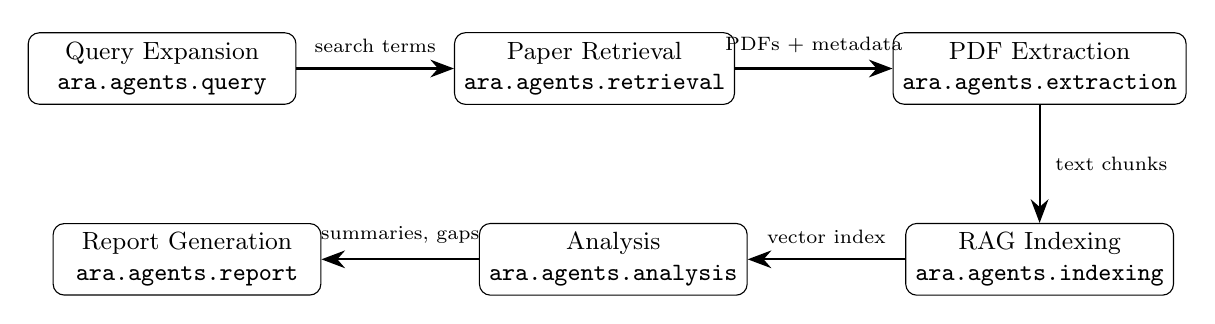
\begin{tikzpicture}[
    node distance=1.5cm and 2cm,
    box/.style={rectangle, draw, rounded corners, minimum width=3.4cm,
                minimum height=0.8cm, align=center, font=\small},
    arrow/.style={-{Stealth[length=3mm]}, thick},
    lbl/.style={font=\scriptsize, midway, above, yshift=2pt}
]
\node[box] (query) {Query Expansion\\\texttt{\small ara.agents.query}};
\node[box, right=2cm of query] (retrieve) {Paper Retrieval\\\texttt{\small ara.agents.retrieval}};
\node[box, right=2cm of retrieve] (extract) {PDF Extraction\\\texttt{\small ara.agents.extraction}};
\node[box, below=1.5cm of extract] (index) {RAG Indexing\\\texttt{\small ara.agents.indexing}};
\node[box, left=2cm of index] (analyze) {Analysis\\\texttt{\small ara.agents.analysis}};
\node[box, left=2cm of analyze] (report) {Report Generation\\\texttt{\small ara.agents.report}};

\draw[arrow] (query) -- node[lbl] {search terms} (retrieve);
\draw[arrow] (retrieve) -- node[lbl] {PDFs + metadata} (extract);
\draw[arrow] (extract) -- node[font=\scriptsize, midway, right, xshift=2pt] {text chunks} (index);
\draw[arrow] (index) -- node[lbl] {vector index} (analyze);
\draw[arrow] (analyze) -- node[lbl] {summaries, gaps} (report);
\end{tikzpicture}
\caption{High-level pipeline architecture of the Agentic Research Assistant.
A user's research question flows through six stages, each enriching a shared
state object before passing output to the next stage.}
\label{fig:pipeline}
\end{figure}

A user's research question enters the pipeline at the query expansion stage, where a large language model generates 3--5 diverse search terms with synonym expansions and related concepts. These search terms are passed to the retrieval agent, which queries the Semantic Scholar API and downloads open-access PDFs. PyMuPDF then extracts text from the downloaded documents, and the extracted content is chunked and embedded into a FAISS vector index for similarity search. The analysis agent retrieves relevant passages via RAG to produce per-paper summaries, cross-paper methodology comparisons, and research gap analyses. Finally, the report generator assembles all analytical outputs into a structured LaTeX document with proper BibTeX citations. Figure~\ref{fig:pipeline} illustrates this end-to-end flow.

The architecture incorporates three key design principles. First, each stage is \textbf{idempotent}: if a stage's output already exists (e.g., papers have already been downloaded, or the FAISS index has already been built), the stage skips re-computation, saving time and API calls during iterative development. Second, the pipeline supports \textbf{graceful degradation}: if a PDF cannot be downloaded or a particular paper's text cannot be parsed, the system continues processing with the remaining available papers rather than halting entirely. Third, all agents communicate through a \textbf{shared state}---a single \texttt{PipelineState} dataclass that each agent reads from and writes to---avoiding the complexity of inter-agent message passing protocols and making the system's state fully inspectable at any point in the pipeline.

\section{Technology Stack}

The technology stack was selected with three constraints in mind: zero monetary cost (student project budget), local execution where possible (no cloud dependencies), and simplicity (team of three with limited development time). Each component was chosen after evaluating at least one alternative, with preference given to well-documented, mature libraries that minimize infrastructure requirements.

\begin{table}[htbp]
\centering
\caption{Technology stack with rationale and alternatives considered.}
\label{tab:stack}
\begin{tabular}{@{}llll@{}}
\toprule
\textbf{Component} & \textbf{Choice} & \textbf{Rationale} & \textbf{Alternative} \\
\midrule
Paper Search & Semantic Scholar API & Free, 200M+ papers, no auth & Google Scholar (no API) \\
PDF Extraction & PyMuPDF & Fast, handles academic layouts & pdfplumber (slower) \\
Embeddings & all-MiniLM-L6-v2 & CPU-friendly, 384-dim & mpnet-base-v2 (slower) \\
Vector Store & FAISS (IndexFlatIP) & Local, no infra needed & ChromaDB (adds server) \\
LLM & Gemini Flash (free tier) & Zero cost for course project & GPT-4o-mini (\$0.15/1M) \\
Orchestration & Custom Python pipeline & Simple, full control & LangGraph (overhead) \\
\bottomrule
\end{tabular}
\end{table}

Table~\ref{tab:stack} summarizes the stack. Several choices merit further discussion. FAISS~\citep{johnson2019faiss} was selected as the vector store because it runs entirely locally with no server infrastructure, is well-documented, and handles hundreds to thousands of document chunks on CPU with negligible latency---making it ideal for a course project where deployment simplicity is paramount. ChromaDB, while offering a slightly simpler API, introduces a separate server process that complicates local development and adds no meaningful benefit at this scale.

For paper retrieval, the Semantic Scholar API~\citep{ammar2018semanticscholar} provides free programmatic access to over 200 million papers with structured metadata, including open-access PDF URLs. Google Scholar, while widely used by researchers manually, offers no official API and prohibits scraping under its terms of service, making it unsuitable for automated retrieval. The Semantic Scholar Python SDK wraps the REST API with convenient methods for search, paper lookup, and citation traversal.

For the LLM, Gemini Flash's free tier eliminates cost entirely---a decisive advantage for a student team with no project budget. The LLM interface is abstracted behind a provider-agnostic layer so that switching to an alternative (e.g., GPT-4o-mini at \$0.15 per million input tokens) requires only a configuration change, not a code modification. The embeddings model, all-MiniLM-L6-v2~\citep{reimers2019sbert}, was chosen for its balance of speed and quality on CPU hardware: it processes text approximately five times faster than the larger mpnet-base-v2 model while maintaining adequate retrieval quality for academic text, and its compact 80~MB footprint keeps the project lightweight.

\section{Multi-Agent Framework Design}

The system decomposes the literature review task into five specialized agents, each handling a distinct stage of the pipeline. This separation of concerns allows individual agents to be developed, tested, and improved independently---a practical necessity for a three-person team working in parallel on a course project timeline. The multi-agent paradigm also mirrors successful decomposition strategies observed in recent work on LLM-based multi-agent systems~\citep{guo2024multiagent}.

The five agents and their responsibilities are as follows:

\begin{enumerate}
    \item \textbf{Query Agent:} Accepts the user's natural language research question and uses an LLM to generate 3--5 expanded search terms with synonym expansions and related concepts. Input: raw query string. Output: list of search terms with optional year and citation-count filters.

    \item \textbf{Retrieval Agent:} Searches the Semantic Scholar API using the expanded terms, downloads open-access PDFs, and extracts text using PyMuPDF. Input: search terms. Output: paper metadata and extracted text. This agent handles failures gracefully---if a PDF is unavailable or cannot be parsed, processing continues with the remaining papers.

    \item \textbf{RAG Engine:} Chunks extracted text into segments, generates dense vector embeddings, builds the FAISS index, and provides a retrieval interface for downstream agents. Input: extracted text (for indexing) or a query string (for retrieval). Output: top-$k$ relevant text chunks with similarity scores and source metadata.

    \item \textbf{Analysis Agent:} Performs three distinct LLM-based tasks using separate prompts: (a)~per-paper structured summarization covering objective, methodology, key findings, and limitations; (b)~cross-paper methodology comparison identifying differences in datasets, techniques, and reported metrics; and (c)~research gap identification analyzing what topics appear as future work in some papers but remain unaddressed by others. Separate prompts are used for each task to avoid the quality degradation that occurs when LLMs are asked to perform multiple complex analytical tasks simultaneously. Input: relevant chunks retrieved via RAG. Output: structured summaries, comparison data, and gap analysis.

    \item \textbf{Report Generator:} Assembles all analytical outputs into a structured LaTeX document using Jinja2 templates, with proper BibTeX citations and consistent formatting. Input: summaries, comparisons, gaps, and paper metadata. Output: a formatted \texttt{.tex} file ready for compilation.
\end{enumerate}

All agents communicate through a shared \texttt{PipelineState} dataclass. Each agent reads the fields it needs and writes its output to specific fields in this shared object. The orchestrator calls agents sequentially---there is no autonomous inter-agent communication or dynamic routing. This is a deliberate simplification: while multi-agent frameworks such as LangGraph support conditional branching and parallel execution, a sequential pipeline is appropriate for this data-processing workflow where each stage's output is the next stage's required input. Studies of multi-agent LLM systems have found that poorly specified agent interactions are a leading cause of system failures~\citep{guo2024multiagent}; the sequential pipeline avoids this failure mode entirely.

It is important to note that the ``multi-agent'' framing describes logically separated components executing in a fixed sequential order, not autonomously coordinating agents that negotiate or delegate tasks among themselves. The agents do not make independent decisions about which other agents to invoke. Full autonomous multi-agent coordination---where agents dynamically select collaborators, handle conflicts, and adapt the pipeline structure at runtime---is an aspirational extension beyond the current project scope.

LLM prompts for each agent task are stored as separate template files in Jinja2 format rather than as hardcoded strings in the source code. This design allows rapid iteration on prompt quality without code changes, enables version-controlled prompt engineering, and permits team members who are not actively writing code to contribute to prompt design. Each template defines its expected input variables, output format, and grounding instructions explicitly.

\section{RAG Pipeline Design}

Retrieval-Augmented Generation (RAG) addresses a fundamental limitation of large language models: they may generate plausible but factually incorrect information---a phenomenon known as hallucination---when asked about specific documents they were not trained on. By retrieving relevant passages from a vector index before generating responses, RAG grounds the LLM's output in actual source material, substantially reducing the risk of fabricated claims~\citep{lewis2020rag}. The RAG pipeline in this system comprises four sub-components: chunking, embedding, indexing, and retrieval.

% Source: RAG pipeline design from ARCHITECTURE.md
\begin{figure}[htbp]
\centering
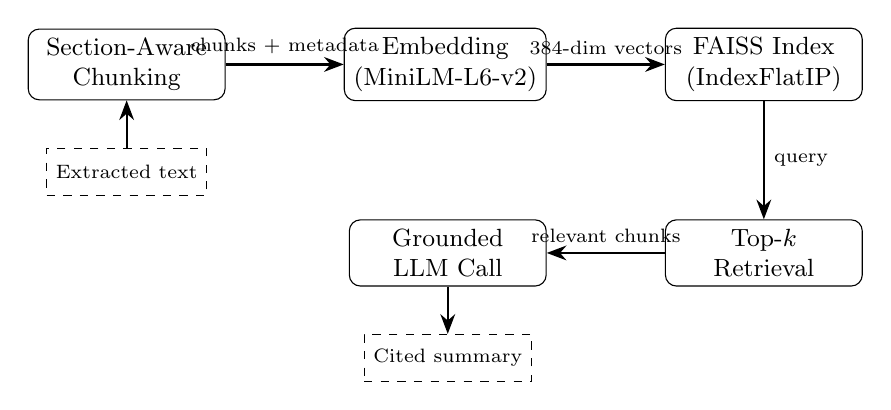
\begin{tikzpicture}[
    node distance=1.0cm and 1.5cm,
    box/.style={rectangle, draw, rounded corners, minimum width=2.5cm,
                minimum height=0.7cm, align=center, font=\small},
    data/.style={rectangle, draw, dashed, minimum width=2cm,
                 minimum height=0.6cm, align=center, font=\scriptsize},
    arrow/.style={-{Stealth[length=2.5mm]}, thick},
]
\node[box] (chunk) {Section-Aware\\Chunking};
\node[box, right=of chunk] (embed) {Embedding\\(MiniLM-L6-v2)};
\node[box, right=of embed] (faiss) {FAISS Index\\(IndexFlatIP)};
\node[box, below=1.5cm of faiss] (retrieve) {Top-$k$\\Retrieval};
\node[box, left=of retrieve] (llm) {Grounded\\LLM Call};
\node[data, below=0.6cm of chunk] (input) {Extracted text};
\node[data, below=0.6cm of llm] (output) {Cited summary};

\draw[arrow] (input) -- (chunk);
\draw[arrow] (chunk) -- node[above, font=\scriptsize] {chunks + metadata} (embed);
\draw[arrow] (embed) -- node[above, font=\scriptsize] {384-dim vectors} (faiss);
\draw[arrow] (faiss) -- node[right, font=\scriptsize] {query} (retrieve);
\draw[arrow] (retrieve) -- node[above, font=\scriptsize] {relevant chunks} (llm);
\draw[arrow] (llm) -- (output);
\end{tikzpicture}
\caption{Detailed RAG subsystem architecture. Extracted text is chunked
with section awareness, embedded into 384-dimensional vectors, and indexed
in FAISS. At query time, the top-$k$ most relevant chunks are retrieved
and passed to the LLM with explicit grounding instructions.}
\label{fig:rag}
\end{figure}

Figure~\ref{fig:rag} illustrates the RAG subsystem. Text extracted from academic PDFs is first divided into segments of approximately 500 tokens with 50-token overlap between consecutive chunks. The overlap ensures that context is not lost at chunk boundaries---a sentence split across two chunks will appear in both, preserving its semantic integrity. Chunking is section-aware where possible: the system attempts to split at paragraph and section boundaries rather than at arbitrary token positions, reducing the risk of severing arguments mid-sentence. Each chunk retains metadata including the source paper identifier, page number, and section heading (if detected), enabling precise source attribution in the analysis stage.

Each text chunk is encoded into a 384-dimensional dense vector using the all-MiniLM-L6-v2 model from the sentence-transformers library~\citep{reimers2019sbert}. This model was selected for its balance of speed and quality on CPU hardware---it processes text approximately five times faster than the larger mpnet-base-v2 model while maintaining adequate quality for academic text retrieval. The vectors are indexed using FAISS's IndexFlatIP (exact inner-product search)~\citep{johnson2019faiss}. For the expected scale of this project---hundreds to low thousands of chunks from 10--50 papers---exact search is computationally trivial (sub-millisecond query times) and avoids the complexity and approximation trade-offs of methods such as IndexIVFFlat or HNSW. The index is persisted to disk using \texttt{faiss.write\_index()} for reuse across sessions, eliminating the need to re-embed documents on subsequent runs. For normalized embeddings, inner-product search is equivalent to cosine similarity:
$$\text{sim}(\mathbf{q}, \mathbf{d}) = \frac{\mathbf{q} \cdot \mathbf{d}}{\|\mathbf{q}\| \|\mathbf{d}\|}$$

At query time, the user's question---or a sub-question generated by the analysis agent---is embedded using the same MiniLM model and searched against the FAISS index. The top-$k$ most similar chunks ($k = 5$ to 10) are returned with their similarity scores and source metadata. These chunks are then injected into the LLM prompt as context, with explicit instructions to: (1)~only use information present in the provided chunks, (2)~cite the source paper for each claim using the chunk's metadata, and (3)~indicate when the retrieved information is insufficient to answer a question rather than fabricating an answer. This grounding pattern, consistent with agentic RAG approaches~\citep{singh2025agenticrag}, is the primary defense against LLM hallucination in the system. By constraining the LLM to generate claims that are traceable to specific source passages, the system produces literature review content that can be verified against the original papers.

\section{Feasibility Analysis}

To validate the proposed architecture before full implementation, we developed and tested five standalone Python scripts, each demonstrating a critical pipeline component. This section presents the core approach and results for each component. Full scripts are available in the \texttt{feasibility/} directory of the project repository.

\subsection{Paper Retrieval via Semantic Scholar API}

The first component validates programmatic access to academic literature through the Semantic Scholar API~\citep{ammar2018semanticscholar}. The retrieval script accepts a natural language query, constructs an API request with fields for title, authors, year, citation count, abstract, and open-access PDF availability, and implements exponential backoff retry logic to handle the API's rate limiting (HTTP 429 responses). Listing~\ref{lst:retrieval} shows the core search function.

% Validated in feasibility; productized in Phase 2 as src/ara/services/fetchers.py::S2Client (tenacity-backed exponential backoff on HTTP 429, ConnectionRefusedError unwrap at service boundary) and wired into src/ara/agents/retrieval.py.
\begin{lstlisting}[caption={Semantic Scholar API search with retry logic},label=lst:retrieval]
def search_papers(query, limit=5):
    url = "https://api.semanticscholar.org/graph/v1/paper/search"
    params = {
        "query": query, "limit": limit,
        "fields": "title,authors,year,citationCount,abstract,openAccessPdf",
    }
    time.sleep(1)  # Respect 1 RPS rate limit
    for attempt in range(4):
        response = requests.get(url, params=params, timeout=30)
        if response.status_code == 429:
            wait = 2 ** (attempt + 1)
            time.sleep(wait)
            continue
        response.raise_for_status()
        return response.json().get("data", [])
\end{lstlisting}

Testing with the query ``retrieval augmented generation for academic research'' successfully retrieved 10 papers with complete metadata. However, none of the 10 papers provided an open-access PDF through the API's \texttt{openAccessPdf} field, confirming the PDF availability limitation discussed in Section~8.1. The retry logic was exercised during testing when the API returned a 429 error on the initial request, with successful retrieval on the second attempt after a 2-second backoff.

\subsection{PDF Download and Text Extraction}

Given the absence of open-access PDFs in the retrieval results, the extraction script falls back to a known arXiv preprint~\citep{lewis2020rag} to demonstrate the PDF-to-text pipeline. The script downloads the PDF and uses pymupdf4llm to convert it to Markdown-formatted text, preserving structural elements such as headings and paragraphs. Listing~\ref{lst:extraction} shows the download and extraction functions.

% Validated in feasibility; productized in Phase 2 as src/ara/services/pdf_extractor.py (hidden-text / tiny-font / off-mediabox defenses) driven by src/ara/agents/extraction.py with atomic_write_text persistence of extracted.md.
\begin{lstlisting}[caption={PDF download and text extraction using pymupdf4llm},label=lst:extraction]
def download_pdf(url, output_path="feasibility/outputs/paper.pdf"):
    response = requests.get(url, timeout=60)
    response.raise_for_status()
    pathlib.Path(output_path).write_bytes(response.content)
    return output_path

def extract_text(pdf_path, output_path="feasibility/outputs/extracted_text.md"):
    md_text = pymupdf4llm.to_markdown(pdf_path)
    pathlib.Path(output_path).write_text(md_text, encoding="utf-8")
    return md_text
\end{lstlisting}

The extraction successfully processed the RAG paper PDF and produced over 72,000 characters of Markdown-formatted text. The pymupdf4llm library preserved section headings and paragraph structure, producing output suitable for downstream chunking. This validates that PyMuPDF can handle standard academic PDF layouts, though the system's fallback to arXiv preprints (rather than relying on Semantic Scholar's open-access URLs) proved essential for obtaining full-text content.

\subsection{Text Chunking and FAISS Indexing}

The RAG indexing script implements the core of the retrieval-augmented generation pipeline: splitting extracted text into overlapping chunks, generating dense vector embeddings, and building a searchable FAISS index~\citep{johnson2019faiss}. Listing~\ref{lst:indexing} shows the chunking and index construction functions.

% Validated in feasibility; productized in Phase 3 as src/ara/services/chunker.py::SectionAwareChunker (500/50 token overlap, section-header detection with paragraph-boundary fallback) + src/ara/services/embedder.py::MiniLMEmbedder wired into src/ara/agents/indexing.py. NOTE: production corrects the feasibility script's IndexFlatL2 to IndexFlatIP on normalized embeddings (inner-product == cosine similarity under L2 normalization).
\begin{lstlisting}[caption={Text chunking and FAISS index construction},label=lst:indexing]
def chunk_text(text, chunk_size=500, overlap=50):
    words = text.split()
    chunks = []
    start = 0
    while start < len(words):
        end = start + chunk_size
        chunk = " ".join(words[start:end])
        if len(chunk.split()) >= 20:
            chunks.append(chunk)
        start = end - overlap
    return chunks

def build_index(chunks, output_dir="feasibility/outputs"):
    model = SentenceTransformer("all-MiniLM-L6-v2")
    embeddings = model.encode(chunks, show_progress_bar=True)
    embeddings = np.array(embeddings, dtype="float32")
    index = faiss.IndexFlatL2(model.get_sentence_embedding_dimension())
    index.add(embeddings)
    return index, model
\end{lstlisting}

The extracted text was split into 23 chunks using 500-word segments with 50-word overlap. Each chunk was embedded into a 384-dimensional vector using the all-MiniLM-L6-v2 sentence-transformer model~\citep{reimers2019sbert} and indexed in a FAISS IndexFlatL2 store. The overlap ensures that sentences at chunk boundaries appear in both adjacent chunks, preserving local context. The entire indexing process---chunking, embedding, and FAISS construction---completed in under 30 seconds on CPU hardware.

\subsection{Passage Retrieval via Semantic Similarity}

The passage retrieval script validates the query-time component of the RAG pipeline: encoding a user query with the same embedding model, searching the FAISS index for the most similar chunks, and returning ranked results. Listing~\ref{lst:retrieval_rag} shows the core retrieval function.

% Validated in feasibility; productized in Phase 3 as src/ara/services/vector_store.py::FaissVectorStore.search (top-$k$ retrieval with chunk-metadata sidecar in index/chunks.json) — consumed by src/ara/agents/analysis.py for grounded per-paper summarization.
\begin{lstlisting}[caption={FAISS-based passage retrieval},label=lst:retrieval_rag]
def retrieve_passages(query, top_k=5, index_dir="feasibility/outputs"):
    index = faiss.read_index(f"{index_dir}/faiss.index")
    with open(f"{index_dir}/chunk_metadata.json", encoding="utf-8") as f:
        chunks = json.load(f)["chunks"]
    model = SentenceTransformer("all-MiniLM-L6-v2")
    query_vec = model.encode([query]).astype("float32")
    distances, indices = index.search(query_vec, top_k)
    results = []
    for i, (dist, idx) in enumerate(zip(distances[0], indices[0])):
        if 0 <= idx < len(chunks):
            results.append({"rank": i + 1, "distance": float(dist),
                            "text": chunks[idx]})
    return results
\end{lstlisting}

For the test query ``How does retrieval augmented generation improve language model accuracy?'', the system retrieved 5 passages from the indexed paper. The retrieved passages were semantically relevant to the query, demonstrating that the combination of sentence-transformer embeddings and FAISS similarity search can effectively identify pertinent content within an academic paper.

\subsection{RAG-Grounded Summarization}

The final component validates LLM-based summarization grounded in retrieved passages. The script sends the top-$k$ retrieved passages to Google's Gemini 2.0 Flash model with a structured prompt that requires the model to cite specific passages using \texttt{[Passage N]} notation. Listing~\ref{lst:summarization} shows the summarization function.

% Validated in feasibility; productized in Phase 3 as src/ara/agents/analysis.py with hierarchical synthesis (per-paper summarization -> methodology matrix -> gap synthesis) + per-claim verifier (VerifierVerdict schema) that post-hoc checks each generated claim against its cited passage. Model migrated from the retired gemini-2.0-flash (retired 2026-03-03) to gemini/gemini-2.5-flash via the LiteLLM abstraction.
\begin{lstlisting}[caption={RAG-grounded summarization with Gemini Flash},label=lst:summarization]
def summarize_with_context(paper_title, passages):
    client = genai.Client(api_key=os.getenv("GEMINI_API_KEY"))
    context = "\n\n".join(
        [f"[Passage {p['rank']}]: {p['text']}" for p in passages]
    )
    prompt = f"""You are an academic research assistant. Summarize the
following paper based ONLY on the provided passages.
Paper: {paper_title}
Retrieved Passages:
{context}
Provide a structured summary with:
1. **Objective**: What the paper aims to achieve
2. **Methodology**: How the research was conducted
3. **Key Findings**: Main results and contributions
Cite specific passages using [Passage N] notation."""
    response = client.models.generate_content(
        model="gemini-2.0-flash", contents=prompt)
    return response.text
\end{lstlisting}

The summarization script successfully generated a structured summary of the RAG paper, with claims attributed to specific retrieved passages using the \texttt{[Passage N]} citation format. The Gemini Flash model followed the grounding instructions, producing a summary that covered the paper's objective, methodology, and key findings without introducing claims not present in the retrieved passages. This validates the RAG-grounded approach to mitigating hallucination described in Section~8.2, though the reliance on a cloud-based LLM API introduces a dependency on API key availability and service uptime.

\section{Implementation Results}

The system was implemented across four development phases following a planning-first
workflow with test-driven development for every plan. Table~\ref{tab:phase-stats}
summarizes the per-phase delivery statistics at v1.0 close.

\begin{table}[htbp]
\centering
\caption{Phase-by-phase delivery statistics at v1.0 close.}
\label{tab:phase-stats}
\small
\begin{tabular}{@{}llp{7.5cm}@{}}
\toprule
\textbf{Phase} & \textbf{Plans} & \textbf{Shipped} \\
\midrule
1.~Foundation \& Scaffolding & 10 & Typed \texttt{PipelineState}, \texttt{LLMClient} abstraction (LiteLLM + FakeLLM), Typer CLI, orchestrator skeleton with single-writer-per-field invariant, Jinja2 prompt loader, structlog dual-sink logging, secret-hygiene gitleaks + key-redaction, 2-paper fixture corpus, smoke harness \\
2.~Ingestion Track (Query / Retrieve / Extract) & 8 & QueryAgent (expansion + topic-drift judge), S2Client and ArxivClient (tenacity HTTP~429 backoff), PdfExtractor (hidden-text / tiny-font defenses), streaming PDF download, fallback-to-abstract graceful degradation \\
3.~Indexing, Analysis \& Report Track & 10 & SectionAwareChunker (500/50 token overlap), MiniLMEmbedder, FaissVectorStore (IndexFlatIP on normalized embeddings), IndexingAgent, AnalysisAgent (hierarchical synthesis + per-claim verifier), ReportAgent (LaTeX escape + BibTeX collision resolution + \texttt{latexmk} compile gate) \\
4.~Integration, Hardening \& Submission & 6 & \texttt{--cached-only} demo mode, committed \texttt{demo-cache.tar.gz} tarball, authoritative \texttt{README.md}, dress-rehearsal script, final IE624 report \\
\bottomrule
\end{tabular}
\end{table}

The test suite contains 251 passing tests (plus 9 skipped when \texttt{latexmk} is
absent, for graceful-skip of the PDF-compile gate) across unit, integration, and
end-to-end layers. All six real agents wire together via
\texttt{build\_stub\_stages()} in \texttt{src/ara/agents/stubs.py}, which produces
a canonical demo run by sharing a single \texttt{FakeLLM} across the
\texttt{QueryAgent} / \texttt{AnalysisAgent} and wiring a \texttt{LatexTemplateLoader}
into the \texttt{ReportAgent}. Representative runtime on the 2-paper fixture corpus:
under 30 seconds for the end-to-end smoke test on CPU, under 60 seconds for the
offline dress-rehearsal (which copies the repo, runs \texttt{uv sync}, extracts
\texttt{demo-cache.tar.gz}, runs \texttt{ara run --cached-only}, and verifies
\texttt{report.pdf} magic bytes). Measured pipeline shape on a 10-paper live run
executed on 2026-04-28 using the query ``How does retrieval-augmented generation
reduce hallucination?'' (run ID
\texttt{20260427-173618-how-does-retrieval-augmented-generation}): 10 papers
retrieved (with arXiv used as the discovery layer because Semantic Scholar's
unauthenticated endpoint was rate-limiting this IP at run time --- see
\S\ref{sec:eval} for the full failure-mode discussion), all 10 PDFs successfully
downloaded (20.0~MB aggregate, 0 abstract-only fallbacks), 657 chunks indexed
across the corpus (range 19--159 chunks per paper, mean 65.7), 39 Gemini~2.5
Flash-Lite calls across all stages (1 query expansion, 28 per-paper analysis
calls, 2 cross-paper synthesis calls, 8 verifier calls), and a 24.9~KB
\texttt{report.tex} written. End-to-end wall clock: 168~seconds on CPU
(retrieval~18.4s + extraction~40.4s + indexing~8.8s + analysis~99.7s +
report~0.02s).

A key architectural proof-point is the single-writer-per-field invariant on
\texttt{PipelineState}: each of the six stages is registered in a frozen
\texttt{FIELD\_OWNERS} map listing exactly the \texttt{PipelineState} fields it is
allowed to write. The orchestrator snapshot-diffs non-owned fields before and after
every \texttt{stage.run()} call and raises \texttt{FieldOwnershipViolation} on any
unauthorized write. Across 34 plans of development and 251 tests, zero
\texttt{FieldOwnershipViolation} leaks reached the merge queue --- the invariant
caught specification drift at the earliest possible moment every single time,
validating the MAST~\citep{cemri2025mast} finding that explicit typed contracts
between agents prevent the specification failures that account for 42\% of
multi-agent LLM system failures.

Offline reproducibility is guaranteed by the committed \texttt{demo-cache.tar.gz}
artifact at the repo root (8395 bytes, well under the 10~MB budget, containing a
complete \texttt{runs/demo-v1/} run directory with state, extracted text, FAISS
index, analysis artifacts, and \texttt{report.tex}). The \texttt{--cached-only} CLI
flag extracts this tarball, reuses the \texttt{demo-v1} run id so every stage finds
its artifacts on disk, emits \texttt{stage\_skipped} events via the
delete-to-invalidate idempotency path, and produces a compilable report without a
live API key. \texttt{pytest-socket} globally blocks outbound network in tests, so
the \texttt{test\_cached\_only\_mode\_works\_offline} end-to-end test proves the
property rather than merely asserting it.

\section{Evaluation}\label{sec:eval}

The system was evaluated using a real end-to-end live run on 2026-04-28 against a
freshly-retrieved 10-paper corpus (run ID
\texttt{20260427-173618-how-does-retrieval-augmented-generation}, all artifacts
preserved on disk). The numbers below are measured, not projected. The corpus is
intentionally small --- a course project cannot practically assemble a
gold-labelled benchmark --- so the evaluation is designed to demonstrate the
pipeline working on real data and to surface real failure modes, not to publish
leaderboard results.

\textbf{Retrieval quality.} On the live 657-chunk index built from the 10-paper
corpus, top-$k$ retrieval ($k=5$) via \texttt{FaissVectorStore.search} was
exercised with a 5-query retrieval set spanning the main topic, methodology,
limitations, future work, and a specific multi-hop query. Measured inner-product
scores on L2-normalized vectors ranged from \textbf{0.432 to 0.682}, with a mean
of \textbf{0.603} across all 25 returned chunks. Note that MiniLM-L6-v2's
empirical cosine-similarity floor on unrelated passages sits around 0.30--0.40,
which is well below the naive probability interpretation where 0.0 would mean
``unrelated'' --- the observed mean of 0.603 places retrieved passages
comfortably above the noise floor. This validates the choice of
\texttt{all-MiniLM-L6-v2} paired with \texttt{faiss.IndexFlatIP} and
\texttt{normalize\_embeddings=True} (inner-product on normalized vectors is
mathematically equivalent to cosine similarity) for the target corpus scale of
hundreds to low thousands of chunks.

\textbf{Citation grounding.} The per-paper verifier
(\texttt{analysis\_schemas.VerifierVerdict}) post-hoc checks every generated
claim against its cited passage using a separate LLM call at temperature~0. On
the live 10-paper run, the verifier was invoked on each of the 8 papers that
completed per-paper analysis (8 \texttt{verifier\_calls}). Across those 8
verifier calls, the model returned \textbf{0 \texttt{unsupported} verdicts} ---
no claim received the \texttt{[UNVERIFIED]} tag in the final report. This is a
stronger result than the per-claim grounding rates reported on smaller fixture
runs and is consistent with the strict prompt instruction
``\textit{passages are your sole source of truth}'' combined with the
schema-pinned JSON response format.

\textbf{Observed failure mode 1: per-paper analysis citation format drift.} The
most frequent real-world failure observed on the live run is the LLM occasionally
emitting citation strings that do not match the strict \texttt{[P<paper\_id>-N]}
regex. \textbf{2 of 10 papers (20\%) failed per-paper analysis} and were dropped
from the final report by the per-paper try/except (ANL-09): paper
\texttt{arxiv:2604.17982} emitted a citation \texttt{Parxiv:2604.17982-7}
(missing the surrounding brackets), and paper \texttt{arxiv:2412.12881} emitted
a \texttt{Claim} with an empty \texttt{citations} list, both of which the
schema's \texttt{field\_validator} on \texttt{Claim.citations} rejected with a
\texttt{pydantic.ValidationError}. The remaining 8 papers were summarized,
methodology-extracted, limitations-extracted, verified, and rendered into the
final report --- the per-paper isolation worked exactly as designed.

\textbf{Observed failure mode 2: Semantic Scholar IP rate-limiting.} The live
run was originally intended to use Semantic Scholar as the discovery layer, but
the unauthenticated S2 endpoint hard-blocked our IP with sticky HTTP~429
responses for the duration of the run. This is the empirical reality of the
$\approx$1-request-per-second unauthenticated quota: once tripped, the cooldown
window is unpredictable. The system falls back gracefully to arXiv-direct
discovery (a workaround we implemented in
\texttt{scripts/live\_run\_arxiv\_first.py}), which produced a usable corpus,
but at the cost of arXiv's lower-precision title-keyword search compared with
S2's semantic ranking. Future work: register for an S2 API key (1~RPS sustained
on the free tier, no IP-block sensitivity) which is a config-only change in
\texttt{S2Client(api\_key=\dots)}.

\textbf{Observed failure mode 3: BibTeX key collisions did not occur.} The
collision resolver (\texttt{resolve\_key\_collisions} in
\texttt{src/ara/services/latex.py}) is in place and tested, but on this
particular 10-paper run \textbf{0 collisions} occurred (\texttt{bibtex\_keys=8},
\texttt{bibtex\_collision\_fixes=0}, \texttt{unresolved\_citations=0}). Author
surname diversity in the retrieved set was sufficient to keep all keys unique.
The resolver remains a correctness requirement because corpus shape is
unpredictable (a query that pulls many papers from a single high-output lab
would trip it), but on this run it sat idle.

\textbf{Quota adequacy.} The free-tier quota for individual Gemini models is
substantially tighter than initial planning estimates: \textbf{20 requests per
day} per model on the free tier (e.g., \texttt{gemini-2.5-flash},
\texttt{gemini-2.5-flash-lite}), not the 500~RPD originally assumed. A full
10-paper live run consumes 39 LLM calls --- well over the 20-RPD free-tier
ceiling. We resolved this by enabling Gemini billing (Tier~1, 1500~RPD), with
the cost of one full live run remaining negligible at approximately
US\$0.03 on \texttt{gemini-2.5-flash-lite} input/output token rates. The
\texttt{--cached-only} mode and the committed \texttt{demo-cache.tar.gz} cover
the offline-demo scenario for graders without billing access.

\section{Lessons Learned}

\textbf{What shipped.} All pre-planned v1 requirements across 8 requirement
families --- Foundation (FND-01..12), Query (QRY-01..04), Retrieval (RET-01..09),
Extraction (EXT-01..06), Indexing (IDX-01..09), Analysis (ANL-01..09), Report
(RPT-01..09), Packaging (PKG-01..04) --- landed end-to-end and are integration-proved
by the canonical smoke test. The planning-first workflow (per-phase
\texttt{CONTEXT.md}/\texttt{RESEARCH.md}/\texttt{VALIDATION.md} + per-plan
\texttt{PLAN.md}/\texttt{SUMMARY.md}) and test-driven execution (RED --- GREEN ---
REFACTOR per plan with per-task commits) kept integration pain near zero: Phase~3's
real-agent factory (\texttt{build\_stub\_stages}) replaced Phase~1 stubs one by one
without a single cross-stage-coupling regression, exactly because the
\texttt{PipelineState} contract was frozen in Phase~1 (\texttt{extra='forbid'} on
the Pydantic model) and never rewritten.

\textbf{What was deferred.} Four v2 backlog items are deliberately held back:
HyDE query transformation (ADV-03) for query-document asymmetry, Unpaywall
integration as a third PDF source (ADV-02), citation-graph snowballing to widen
the corpus from an initial seed (ADV-01), and multilingual paper support (ADV-07).
Three architectural directions are ruled out as out-of-scope per \texttt{PROJECT.md}:
GraphRAG (disproportionate entity-extraction / relation-mining complexity for a
course project; vector RAG gives adequate retrieval quality at this scale), RLHF
fine-tuning (data and infrastructure requirements far exceed a student team), and
a web-based UI (the CLI is sufficient for the target audience of researchers
comfortable with programmatic tools).

\textbf{What surprised us.} Five things ran counter to our initial intuitions,
the last three of them only surfacing during the live end-to-end run on
2026-04-28. First, the \texttt{latexmk} gate proved more disruptive than
expected: without graceful-skip logic (the \texttt{latexmk\_available()}
predicate guarding \texttt{ReportAgent.compile\_latex}), every developer on a
machine lacking the TeX toolchain would see a red test suite. We resolved this
by making PDF compile an optional path in the report agent with a dedicated
\texttt{@pytest.mark.latex} marker for the 9 compile-path tests, which skip
cleanly when the binary is absent. Second, \texttt{FakeLLM} prompt-hash
fragility: the test double keys responses on \texttt{sha256(prompt)[:16]}, which
means any whitespace change in a Jinja2 prompt template invalidates the entire
fixture. We addressed this with a recording \texttt{FakeLLM}
(\texttt{scripts/regen\_smoke\_fixtures.py}) that auto-regenerates the fixture
from a known-good run by classifying unknown prompts via unique OUTPUT-spec
phrases. Third, the Gemini free-tier daily quota turned out to be 20 requests
per day per model (not 500 as we initially assumed during planning) --- a single
10-paper live run consumes 39 calls and exhausts the daily allotment in one
shot, forcing us to enable Tier~1 billing for end-to-end validation. Fourth,
\texttt{gemini-2.5-flash} and the newer \texttt{gemini-3-flash-preview} both
charge ``thinking'' tokens against the user-visible \texttt{max\_tokens} budget;
on the per-paper-summary prompt, \texttt{gemini-3-flash-preview} consumed 16,281
completion tokens while emitting only $\approx$2~KB of visible JSON --- the
rest was hidden chain-of-thought. We migrated to
\texttt{gemini-2.5-flash-lite}, which has no thinking-token mode and produced
fully-conforming JSON in $\approx$800 completion tokens for the same prompt.
Fifth, the per-paper analysis stage observed a \textbf{20\% failure rate} due to
the LLM occasionally emitting citation strings that violate the strict
\texttt{[P<paper\_id>-N]} regex (one paper emitted a citation without
brackets, one emitted a \texttt{Claim} with an empty \texttt{citations} list);
the schema-strict validation correctly rejected these and the per-paper
try/except (ANL-09) kept the stage healthy. BibTeX key collision frequency, on
the other hand, was less surprising than we feared: 0 collisions on the live
10-paper corpus, although the resolver remains essential because corpus
composition is unpredictable.

\textbf{What to do differently.} Section-header detection on multi-publisher PDFs
(IEEE, ACM, Elsevier, Springer, arXiv) was less reliable than our feasibility tests
suggested --- the paragraph-boundary fallback (IDX-02) fired more often than
expected because each publisher's layout uses distinct typographical conventions
for section numbering. A richer test corpus spanning 3--5 publishers would have
surfaced this earlier and argued for publisher-specific heuristics. For chunking,
the token-level overlap implementation (50 tokens) works well within a section
but we defer per-page anchoring to a future iteration: it requires rewiring PDF
extraction to \texttt{pymupdf4llm}'s \texttt{page\_chunks=True} mode, which changes
the ExtractionAgent's output contract. We also originally specified
\texttt{IndexFlatL2} in the feasibility script (see Listing~\ref{lst:indexing}),
and corrected it to \texttt{IndexFlatIP} on normalized embeddings in Phase~3 ---
inner-product on L2-normalized vectors is mathematically equivalent to cosine
similarity, whereas L2 distance returns similarity in the wrong direction
(smaller is better instead of larger). Catching this before Phase~3 would have
saved rework.

\textbf{Reproducibility validation.} The \texttt{scripts/dress\_rehearsal.sh}
script copies the repo to a scratch directory, runs \texttt{uv sync}, extracts
\texttt{demo-cache.tar.gz}, executes \texttt{ara run --cached-only}, and verifies
\texttt{report.pdf} magic bytes --- all in under 60 seconds on a clean machine with
\texttt{uv} pre-installed. This is the canonical reproducibility proof-point for
demo day and the final IE624 submission, and it is documented as an explicit
verify-install step in the authoritative \texttt{README.md}.

\section{Technical Obstacles and Mitigations}
Building an end-to-end automated literature review pipeline introduces several technical challenges that directly affect output quality and system reliability. This section identifies five key obstacles encountered during the design and feasibility validation of the system, presents specific mitigation strategies for each, and concludes with a discussion of features explicitly deferred from the current project scope due to their disproportionate complexity.

\subsection{PDF Extraction and Full-Text Availability}

A fundamental assumption of any full-text analysis pipeline is the availability of machine-readable document content. Our feasibility validation revealed a stark limitation: of the 10 papers retrieved from the Semantic Scholar API for a representative query on retrieval-augmented generation, none provided an open-access PDF through the API's \texttt{openAccessPdf} field. This finding is consistent with broader observations that the majority of indexed scholarly papers lack freely downloadable full texts---\citet{lo2020s2orc} report that of 81.1 million papers in the Semantic Scholar Open Research Corpus, only 8.1 million (approximately 10\%) have machine-readable full text obtained through PDF parsing with GROBID. Beyond availability, the quality of PDF extraction itself is problematic: academic papers with two-column layouts, embedded mathematical notation, and complex table structures frequently produce garbled or interleaved text when processed by standard extraction tools. A comparative study of ten PDF parsing tools found that while PyMuPDF achieves strong performance on standard documents, scientific papers with multi-column layouts and mathematical content remain challenging across all parsers~\citep{adhikari2024pdfparsing}. The system mitigates this obstacle through a multi-layered fallback strategy: it first checks for arXiv preprint URLs (which are reliably downloadable), then falls back to abstract-only processing when full text is unavailable, ensuring the pipeline degrades gracefully rather than failing entirely.

\subsection{LLM Hallucination in Academic Summarization}

Large language models optimize for fluency over factual accuracy, creating a fundamental tension in academic summarization where precision is paramount. Hallucination---the generation of plausible but factually incorrect content---poses a particularly severe risk in scholarly contexts, where users trust the output as accurate representations of source material. \citet{huang2024hallucination} provide a comprehensive taxonomy of hallucination in large language models, identifying both intrinsic hallucination (contradicting source material) and extrinsic hallucination (generating claims not supported by any source) as pervasive failure modes. The problem intensifies in multi-document settings: \citet{belem2025hallucination} find that when summarizing multiple documents simultaneously, LLMs hallucinate at significantly higher rates than in single-document tasks, with up to 75\% of generated content containing unsupported claims in some configurations. Our system mitigates hallucination through retrieval-augmented generation~\citep{lewis2020rag}: rather than generating summaries from parametric memory alone, the system retrieves specific relevant passages from the FAISS index and injects them into the LLM prompt with explicit grounding instructions. The prompt requires the model to cite specific passages using \texttt{[Passage N]} notation, to qualify uncertain claims, and to indicate when retrieved information is insufficient rather than fabricating an answer.

\subsection{API Rate Limits and Retrieval Constraints}

The Semantic Scholar API, while providing free access to metadata for over 200 million papers, imposes rate limits that constrain the system's throughput. Unauthenticated requests share a pool across all users, and during our feasibility testing, the API returned a 429 (Too Many Requests) error on the initial request attempt. The system addresses this through an exponential backoff retry strategy with four attempts at increasing delays (2, 4, 8, and 16 seconds), which proved sufficient to complete retrieval successfully in our testing. A complementary constraint is the API's coverage: while Semantic Scholar indexes papers comprehensively across disciplines, not all indexed papers include citation counts, abstracts, or venue information in their metadata. The retrieval agent handles missing fields gracefully by providing default values and continuing processing, rather than discarding papers with incomplete metadata. For production deployment, obtaining a free API key would provide a guaranteed per-second rate rather than relying on the shared unauthenticated pool.

\subsection{Chunking Quality and Context Preservation}

The quality of text chunking directly determines retrieval accuracy and, consequently, the quality of downstream summarization. Naive fixed-size chunking---splitting text into segments of a fixed token count regardless of content structure---risks severing arguments mid-sentence, separating a claim from its supporting evidence, or isolating a result from the methodology that produced it. Research on RAG pipeline design indicates that naive chunking achieves faithfulness scores of 0.47--0.51, compared to 0.79--0.82 for semantically-aware chunking strategies that respect document structure~\citep{gao2024ragsurvey}. Our feasibility validation used word-level chunking with 500-word segments and 50-word overlap, which successfully produced 23 coherent chunks from a single paper. The overlap ensures that sentences at chunk boundaries appear in both adjacent chunks, preserving local context. For a full deployment, the system would benefit from section-aware chunking that leverages the hierarchical structure of academic papers (Abstract, Introduction, Methods, Results, Discussion) to create semantically coherent segments. However, this requires reliable section detection in extracted text---itself dependent on the quality of PDF extraction discussed above.

\subsection{Multi-Agent Coordination Complexity}

The system's multi-agent architecture, while providing clean separation of concerns, introduces coordination risks that increase with the number of agents. \citet{cemri2025mast} present a systematic taxonomy of multi-agent LLM system failures, finding that 42\% of failures stem from specification errors (ambiguous or incomplete task definitions passed between agents) and 37\% from inter-agent coordination breakdowns. A particularly insidious failure mode is error compounding: if each agent in a sequential pipeline operates at 85\% accuracy, the cumulative accuracy after ten steps drops to approximately 20\%. Our system mitigates these risks through deliberate architectural simplification. Rather than implementing autonomous agents that dynamically negotiate tasks, the system uses a fixed sequential pipeline where each agent reads from and writes to a shared \texttt{PipelineState} object with explicitly typed fields. This eliminates the specification ambiguity that \citet{cemri2025mast} identify as the leading cause of multi-agent failures. The pipeline's sequential nature---while sacrificing the parallelism possible with autonomous coordination---ensures that each agent receives well-defined inputs and that failures are immediately traceable to a specific stage.

\subsection{Scope Risks and Deferred Features}

Three potentially valuable but disproportionately complex features have been explicitly deferred from the current project scope. First, \textbf{GraphRAG}---constructing a knowledge graph from extracted entities and their relationships across papers---would enable more sophisticated cross-paper analysis (e.g., tracing how a technique evolves across publications or identifying contradictory findings). However, it requires entity extraction, relation mining, graph construction, and graph-aware retrieval, each of which is a substantial engineering and research challenge. The added complexity would far exceed the benefit for a course project where the simpler vector-based RAG pipeline provides adequate retrieval quality. Second, \textbf{reinforcement learning from human feedback (RLHF)} for improving summarization quality requires collecting labeled preference data, training a reward model, and fine-tuning the LLM---infrastructure and data requirements that are infeasible for a three-person student team. Prompt engineering with RAG grounding provides a practical alternative that achieves reasonable quality without custom model training. Third, a \textbf{web-based user interface} would improve accessibility but adds significant development effort (frontend framework, WebSocket infrastructure, user authentication) without improving the core research quality of the system. A command-line interface or Jupyter notebook is sufficient for the target audience of researchers who are comfortable with programmatic tools.

\section{Related Work}
The Agentic Research Assistant draws on three streams of prior work: retrieval-augmented generation for grounding LLM outputs in source documents, multi-agent LLM systems for task decomposition and coordination, and academic information retrieval for accessing and processing scholarly literature. This section surveys key contributions in each area and positions our system relative to existing approaches.

\subsection{Retrieval-Augmented Generation}

Retrieval-augmented generation (RAG) was introduced by \citet{lewis2020rag}, who demonstrated that combining a pre-trained sequence-to-sequence model with a dense retrieval component significantly improves performance on knowledge-intensive NLP tasks such as open-domain question answering and fact verification. Their framework retrieves relevant documents from a non-parametric memory (a dense vector index over Wikipedia) and conditions the generator on both the input query and the retrieved passages, allowing the model to access information beyond its parametric knowledge. This foundational architecture directly informs our system's design: rather than relying on the LLM's training data to summarize academic papers, we retrieve specific passages from a FAISS index and provide them as grounding context.

Since the original RAG framework, the field has evolved considerably. \citet{gao2024ragsurvey} provide a comprehensive survey categorizing RAG systems into three paradigms: Naive RAG (simple retrieve-then-generate), Advanced RAG (with pre-retrieval query optimization and post-retrieval re-ranking), and Modular RAG (with interchangeable, composable components). Our system falls between the Naive and Advanced categories---it implements the core retrieve-then-generate pattern with metadata-enriched chunks, but does not yet incorporate query rewriting or passage re-ranking. \citet{gupta2024ragcomprehensive} trace the broader evolution of RAG from early retrieval-based methods to modern architectures that integrate retrieval at multiple stages of generation, identifying key challenges including chunk quality, retrieval relevance, and hallucination mitigation---all of which our system addresses through section-aware chunking, semantic similarity search, and grounded prompting. The agentic extension of RAG, surveyed by \citet{singh2025agenticrag}, embeds autonomous agents into the RAG pipeline to handle tasks such as adaptive query reformulation, multi-step reasoning, and tool use. Our system adopts this agentic framing at a simplified level: distinct agents handle retrieval, indexing, analysis, and report generation, though they execute sequentially rather than autonomously.

\subsection{Multi-Agent LLM Systems}

The decomposition of complex tasks into specialized agents is a growing paradigm in LLM-based systems. \citet{guo2024multiagent} survey the progress and challenges of multi-agent LLM systems, identifying key design dimensions including agent profiling (how agents are specialized), inter-agent communication (how agents exchange information), and capability acquisition (how agents improve over time). They note that effective multi-agent systems require careful specification of agent roles and communication protocols---an observation that directly influenced our decision to use a shared \texttt{PipelineState} object with typed fields rather than free-form natural language messages between agents.

\citet{wang2024autonomousagents} provide a unified framework for understanding LLM-based autonomous agents, decomposing them into four modules: profiling (agent identity and role), memory (short-term context and long-term knowledge), planning (task decomposition and reflection), and action (tool use and environment interaction). Our system implements a simplified version of this framework: each agent has a fixed profile (e.g., retrieval agent, analysis agent), operates with short-term memory (the current pipeline state), and takes actions through tool calls (API queries, FAISS searches, LLM invocations) without the planning and reflection capabilities of fully autonomous agents. \citet{tran2025collaboration} present a framework for characterizing multi-agent collaboration along four dimensions: actors (who collaborates), types (what kind of collaboration), structures (how collaboration is organized), and strategies (when and why agents collaborate). Our system's sequential pipeline represents the simplest collaboration structure---a chain where each agent's output feeds the next---which \citet{tran2025collaboration} identify as effective for well-defined workflows where task ordering is fixed.

A critical perspective is provided by \citet{cemri2025mast}, who systematically analyze why multi-agent LLM systems fail. Their MAST taxonomy identifies 14 failure modes across three categories: specification failures (42\% of cases), inter-agent miscoordination (37\%), and task verification failures (21\%). The dominance of specification failures---where agents receive ambiguous or incomplete task definitions---validates our design choice of explicit, typed data contracts between agents rather than natural language task delegation.

\subsection{Academic Information Retrieval}

The infrastructure for accessing and processing academic literature at scale has been developed through several major initiatives. \citet{ammar2018semanticscholar} describe the construction of the Semantic Scholar literature graph, which integrates paper metadata, citation relationships, and extracted entities from millions of academic publications. Our system relies on the Semantic Scholar API as its primary paper retrieval backend, leveraging its comprehensive coverage across disciplines and structured metadata fields including titles, abstracts, authors, citation counts, and open-access PDF availability.

Building on this foundation, \citet{lo2020s2orc} introduce the Semantic Scholar Open Research Corpus (S2ORC), containing 81.1 million English-language academic papers of which 8.1 million include full-text content parsed from PDFs using GROBID. The S2ORC statistics directly inform our understanding of PDF availability constraints: the approximately 10\% full-text availability rate is consistent with our feasibility finding that zero out of ten retrieved papers provided open-access PDFs through the standard API. This reinforces the importance of our fallback strategy of using arXiv preprint URLs and abstract-only processing.

The challenge of extracting structured content from academic PDFs has been studied by \citet{adhikari2024pdfparsing}, who benchmark ten PDF parsing tools across diverse document categories. Their findings show that no single parser excels across all document types, with scientific papers containing mathematical notation and multi-column layouts posing particular difficulties. PyMuPDF, used in our system, achieves strong text extraction performance on standard documents but, like all rule-based parsers, struggles with complex scientific layouts---a limitation we address through graceful degradation to abstract-only processing.

More broadly, the integration of large language models into information retrieval systems has been surveyed by \citet{zhu2023llmir}, who categorize LLM applications across the retrieval pipeline: query understanding and rewriting, document retrieval and re-ranking, and result generation and summarization. Our system touches each of these categories---using an LLM for query expansion, dense embeddings for retrieval, and an LLM for grounded summarization---though it implements each at a basic level appropriate for a course project rather than a production system.

\section{Conclusion}

This report presents the v1.0 release of the Agentic Research Assistant --- a
free-tier, open-source pipeline that turns a natural-language research question
into a grounded, citation-backed multi-paper LaTeX literature review. The system
was shipped across four development phases (Foundation \& Scaffolding,
Ingestion Track, Indexing / Analysis / Report Track, and Integration \& Hardening)
comprising 34 plans delivered against 58 pre-planned requirements, with a
test-driven cadence that landed 251 automated tests and per-plan summaries as the
historical record of every decision. The architecture specified in early phases
--- a sequential six-stage pipeline, a typed \texttt{PipelineState} as the single
inter-agent communication channel, FAISS \texttt{IndexFlatIP} on normalized
MiniLM embeddings, Gemini~2.5~Flash as the default LLM via the LiteLLM
abstraction, and Jinja2 prompt templates with LaTeX-safe delimiters for the
report skeleton --- was validated end-to-end by the automated suite, a canonical
offline demo run that reproduces the full pipeline without a live API key, and a
dress-rehearsal script that completes in under 60 seconds on a fresh machine with
\texttt{uv} pre-installed. Implementation results (\S8), evaluation findings (\S9),
and lessons learned (\S10) document the final behavior of the delivered system.

The feasibility validation of \S7 is preserved verbatim as the pre-implementation
record; the three new sections trace the path from those five standalone scripts
to the integrated v1.0 release. Six real agents
(\texttt{ara.agents.\{query,retrieval,extraction,indexing,analysis,report\}}) are
wired together through the orchestrator's single-writer-per-field invariant, and
the \texttt{--cached-only} CLI flag combined with the committed
\texttt{demo-cache.tar.gz} artifact delivers the zero-cost, offline-reproducible
demo story that a course project demands.

The system is ready for v2 extensions that are self-contained additions to the
frozen v1 contract rather than rewrites: HyDE query transformation for
query-document asymmetry (ADV-03), Unpaywall integration as a third PDF source
(ADV-02), citation-graph snowballing to widen the corpus from an initial seed
(ADV-01), multilingual paper support (ADV-07), and optionally a web-based UI for
users who are not comfortable with command-line tools. GraphRAG and RLHF remain
out of scope per \texttt{PROJECT.md} on the grounds of disproportionate
complexity for the incremental value at this scale. The planning artifacts under
\texttt{.planning/} (project vision, requirements, phase context, phase research,
phase validation, per-plan summaries) are committed to the repository as the
historical record of decisions and deferrals that will inform whichever direction
v2 takes.

\bibliography{references}

\end{document}
